\documentclass{article}
\usepackage[utf8]{inputenc}
\usepackage{graphicx}
\usepackage{karnaugh-map}

\title{Assignment9}
\author{Abhay Suresh}
\date{4th January 2021}

\usepackage{xcolor}
\usepackage{listings}

\definecolor{mGreen}{rgb}{0,0.6,0}
\definecolor{mGray}{rgb}{0.5,0.5,0.5}
\definecolor{mPurple}{rgb}{0.58,0,0.82}
\definecolor{backgroundColour}{rgb}{0.95,0.95,0.92}

\lstdefinestyle{CStyle}{
    backgroundcolor=\color{backgroundColour},
    commentstyle=\color{mGreen},
    keywordstyle=\color{magenta},
    numberstyle=\tiny\color{mGray},
    stringstyle=\color{mPurple},
    basicstyle=\footnotesize,
    breakatwhitespace=false,
    breaklines=true,
    captionpos=b,
    keepspaces=true,
    numbers=left,
    numbersep=5pt,
    showspaces=false,
    showstringspaces=false,
    showtabs=false,
    tabsize=2,
    language=C
}

\begin{document}

\maketitle

\section{Assigned Question}
\begin{figure}[htp]
    \centering
    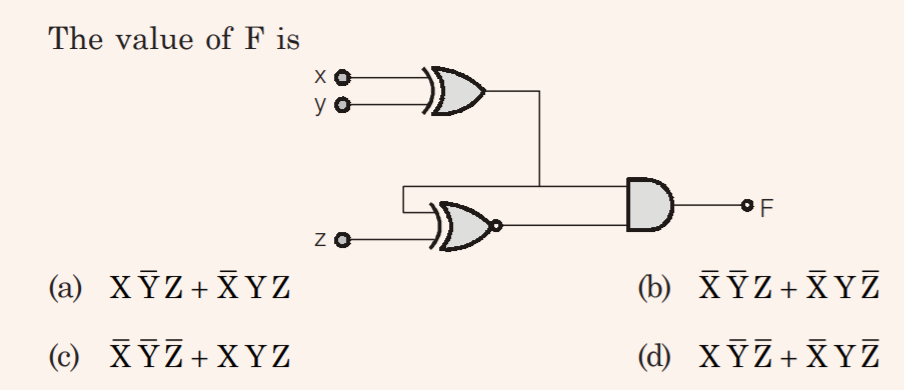
\includegraphics[width=13cm]{A9.png}
\end{figure}
\section {Solution - Forming the Boolean Equation}
\\
From the Given logic gate we can identify three different logic gates XOR, XNOR and AND gate using X,Y,Z as variables and F as the output.
\\
Let us represent these Logic gates as A and B, as shown in the following figure.

\begin{figure}[htp]
    \centering
    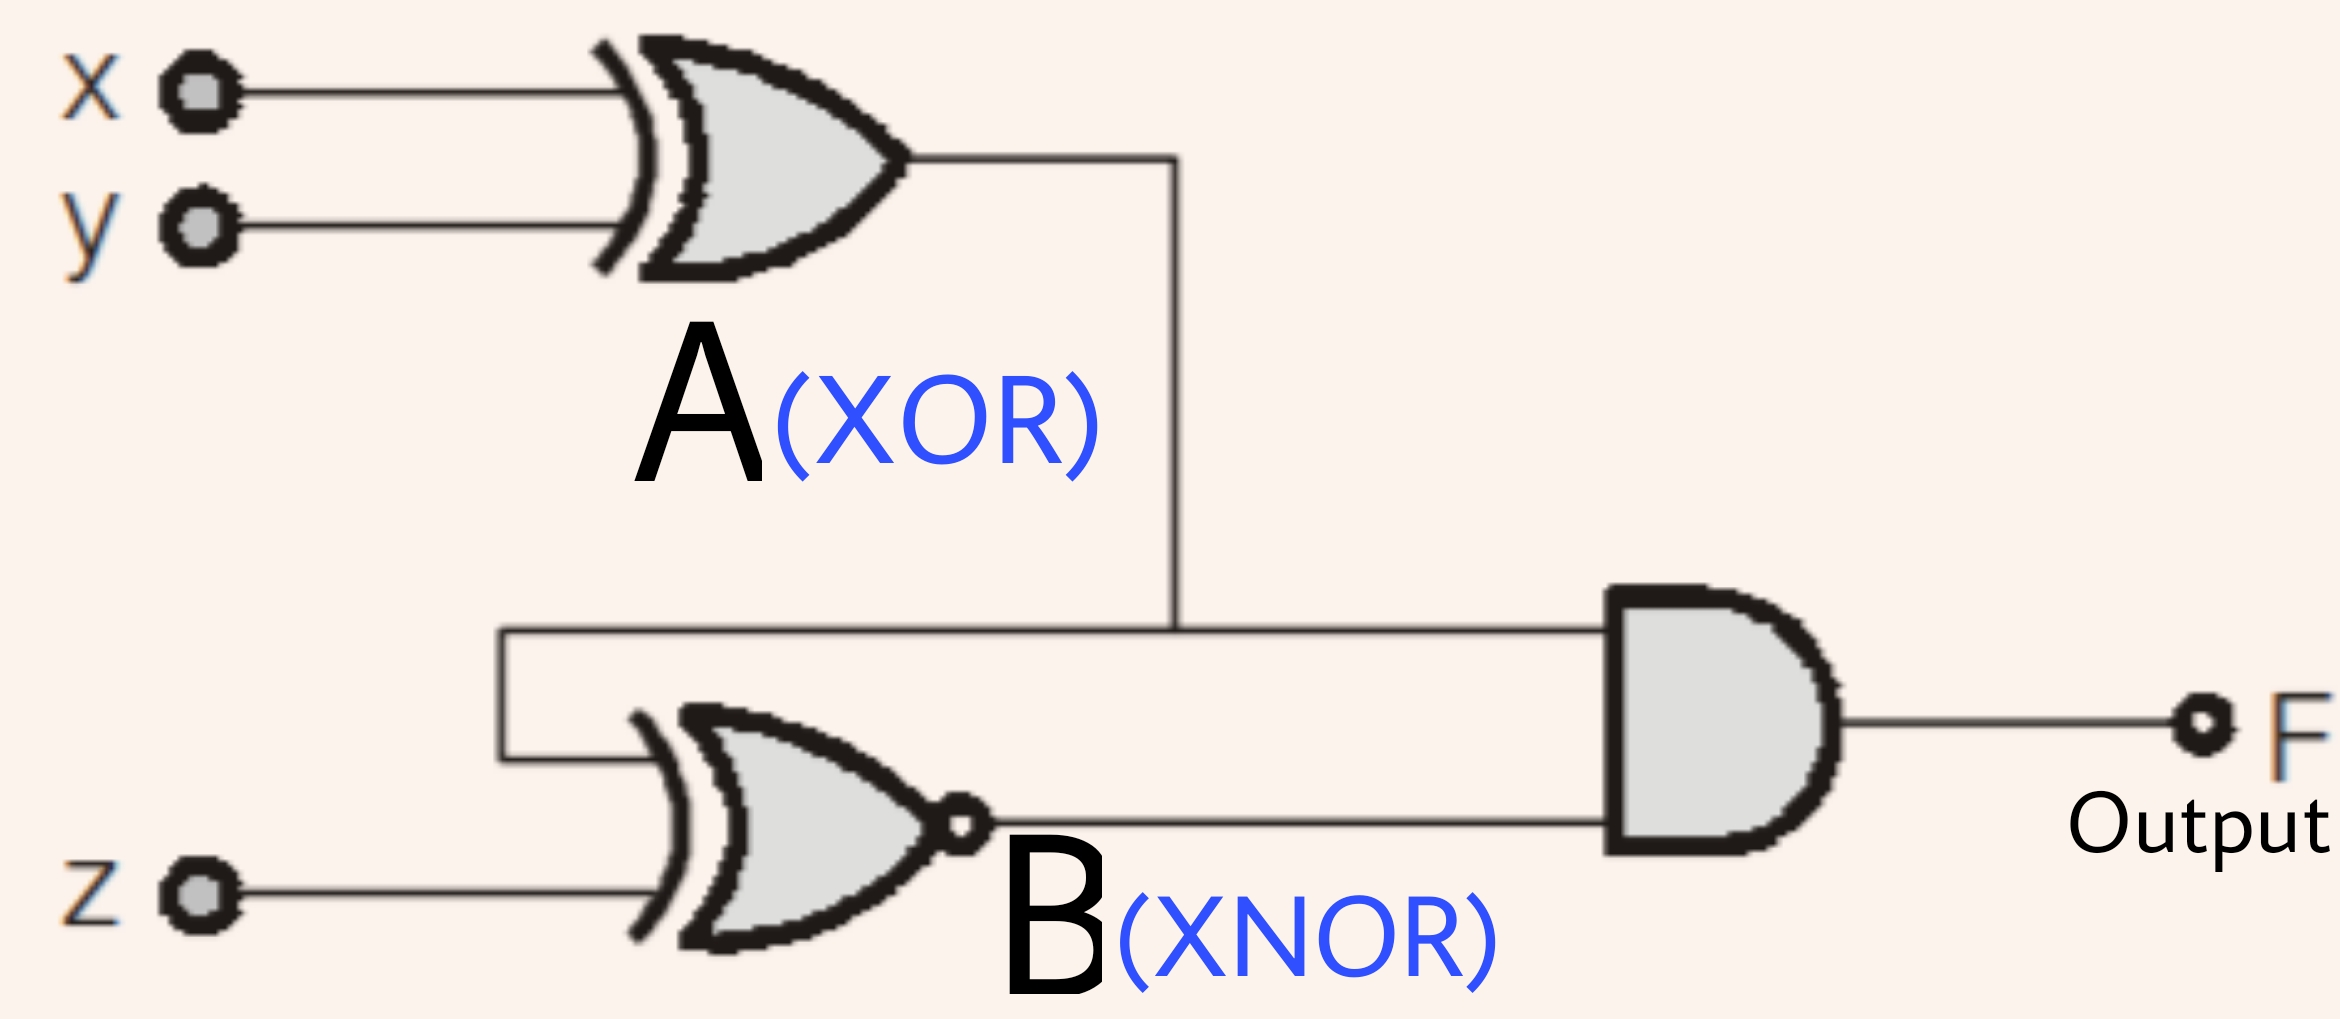
\includegraphics[width=9cm]{AA9.jpg}
\end{figure}
\\
The Output from A (XOR), where X and Y are the inputs, can be written as
\\
\bold $A = (\bar{X}{Y} + {X}\bar{Y})$
\\
\\
Similarly the output from B (XNOR),where A and Z are the inputs can be written as
\\
$B = ({A}{Z} + \bar{A}\bar{Z})$
\\
\\
Now A and B are the inputs for the required Output F which is
\\
$F = ({A}{B})$
\\
\\
From the previously obtained Boolean equations for A and B,
\\$F = [(\bar{X}{Y} + {X}\bar{Y})({(\bar{X}{Y} + {X}\bar{Y})}{Z} + \overline{(\overline{X}{Y} + {X}\overline{Y})}\bar{Z})]$
\\
\\
\section {Truth Values of the Boolean Equation}
The obtained Boolean equation can be simplified further using a K-Map using the Truth Table of the Boolean Equation.
\\
\\
The Truth table values of the boolean equation has been found using a C code for the boolean equation which is mentioned in Section 5
\\
\\
\begin{center}
\begin{tabular}{ |c|c|c|c|c|c| }
\hline
\multicolumn{3}{|c|}{Input}&{XOR Output}&{XNOR Output}&{Final Output}\\
\hline
X&Y&Z&A&B&F = A.B\\
\hline
0&0&0&0&1&0\\
0&0&1&0&0&0\\
0&1&0&1&0&0\\
1&0&0&1&0&0\\
0&1&1&1&1&1\\
1&0&1&1&1&1\\
1&1&0&0&1&0\\
1&1&1&0&0&0\\
\hline
\end{tabular}
\end{center}
\\
\\
\section {Simplified Equation using K-Map}
From the Truth table obtained for the Logic Gates we can Simplify the respective Boolean Equation using K-Map,using the variables X,Y,Z.

\begin{center}
\begin{karnaugh-map}[4][2][1][][]
    \maxterms{0,1,2,4,6,7}
    \minterms{3,5}
    \implicant{3}{3}
    \implicant{5}{5}
    % note: position for start of \draw is (0, Y) where Y is
    % the Y size(number of cells high) in this case Y=2
    \draw[color=black, ultra thin] (0, 2) --
    node [pos=0.7, above right, anchor=south west] {$YZ$} % YOU CAN CHANGE NAME OF VAR HERE, THE $X$ IS USED FOR ITALICS
    node [pos=0.7, below left, anchor=north east] {$X$} % SAME FOR THIS
    ++(135:1);
    \end{karnaugh-map}
    \end{center}

The above obtained K-Map gives two terms in SOP as
\\
$F = (\bar{X}{Y}{Z} + {X}\bar{Y}{Z})$ which is option (a).

\section {C Code used to obtain the Truth Table in \\ Section 3 and Verify the Final Boolean\\ Equation}

\begin{lstlisting}[style=CStyle]
//This C program is used to verify the obtained boolean eq(unsimplified) of the logic gate from Assignment 9 and to derive its Truth Values(EC2014,14)

#include <stdio.h>

//The  main function
int main(void)
{
unsigned char  X=0x01,Y=0x01,Z=0x00;//inputs in hex	
unsigned char one = 0x01;//used for displaying the output in bit
unsigned char A,B,F;//outputs

            A = ((~X)&Y)|((~Y)&X);
            //XOR GATE

            B = (A&Z)|((~A)&(~Z));
            //XNOR GATE

            F = A&B;
            //Final output F (AND GATE)

printf("The following is the Input for the Logic gate for the Assignment 9,represented using X,Y,Z\n\n");
printf("X = %x  Y = %x  Z = %x",one&X,one&Y,one&Z);//Intput XYZ
printf(" \n");
printf("\n The output of the logic gate, ");
printf("F = %x\n" ,one&F);//Output F
printf("  \n");
printf("Similarly,rest of the values of input XYZ has been pre verified using this C program");
return 0;
}

\end{lstlisting}
\end{document}

\end{document}
